\begin{comment}
\begin{frame}[plain]
\begin{center}
\textbf{\Large Calibration des jets}
\end{center}
\end{frame}
\end{comment}

\begin{frame}
\frametitle{Calibration des jets}
\begin{columns}
\begin{column}{0.7\textwidth}
\begin{maliste}
%\item Premières données de 2010 : \textcolor{red}{XX~fb$^{-1}$}
\item Production massive de jets au LHC
\vspace*{0.2cm}
\item Acc\`es aux particules instables : top, W, Higgs, etc.
\vspace*{0.2cm}
\item Nécessité d'une calibration : non-compensation, matériaux morts, out-of-cone, ...
\vspace*{0.2cm}
\item Objet de référence : jet de particules 
\begin{itemize}
%\item Algorithme : \antikt
\item Input : particules stables après hadronisation (sauf muons et neutrinos)
\item \'Energie : \Etruth
\end{itemize}
\end{maliste}
\end{column}
\begin{column}{0.35\textwidth}
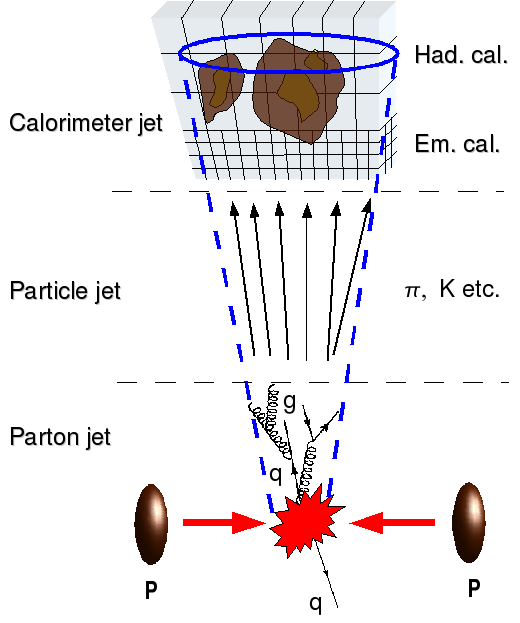
\includegraphics[width=.9\textwidth]{Figures/JES/jetAtVariousLevelIllustration.png}
\end{column}
\end{columns}
\begin{center}
\begin{minipage}{4cm}
\begin{varblock}[5cm]{}
\begin{normalsize}
\textcolor{blue}{Objectifs : $R=\left<E/\Etruth\right>\simeq 1$}
\begin{itemize}
\item \textcolor{blue}{Petite incertitude sur $R$}
\item \textcolor{blue}{Bonne résolution en énergie}
\end{itemize}
\end{normalsize}
\end{varblock}
\end{minipage}
\end{center}
\end{frame}

\begin{frame}
\frametitle{Les 4 calibrations dans ATLAS au d\'ebut du run 1}

\vspace*{-0.3cm}
\begin{columns}
\begin{column}{0.5\textwidth}
\begin{block}{EM+JES}
\begin{itemize}
%\item Calibration la plus simple
\item Apr\`es calibration : $R(p_T,\eta)=1$
\item Constantes d\'eriv\'ees au tout d\'ebut du run 1 (stage M2 J. Demaizi\`ere)
\begin{center}
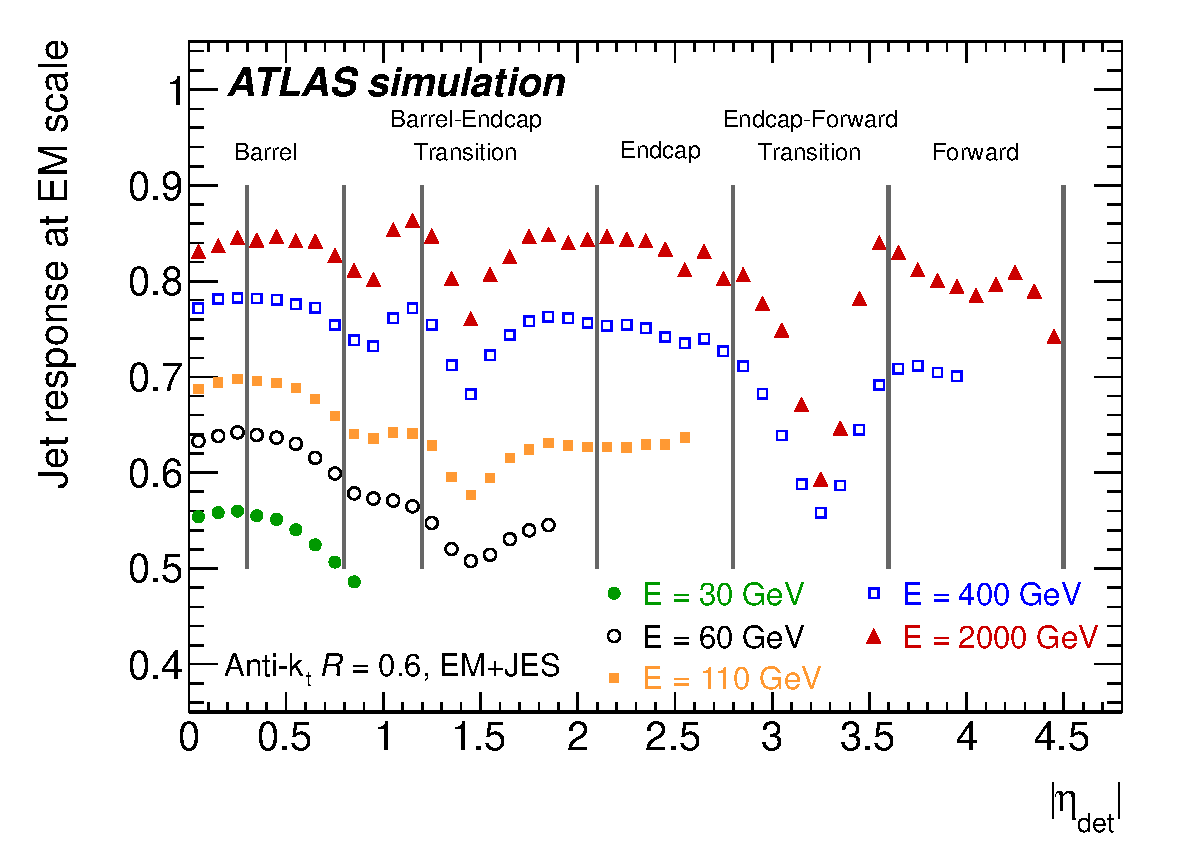
\includegraphics[scale=0.2]{Figures/JES/fig_09_responseEMscaleVsEta.pdf}
\end{center}
\end{itemize}
\end{block}
\end{column}
\pause
\begin{column}{0.55\textwidth}
{
\setbeamercolor{block title}{use=structure,fg=white,bg=green!20!black}
\setbeamercolor{block body}{use=structure,fg=black,bg=green!10!white}
\begin{block}{GCW+JES {\small (``Global Cell Weighting'')}}
\begin{itemize}
\item Principe : calibration bas\'ee sur densit\'e d'\'energie des cellules $E/V$
\item Minimisation \\
\begin{scriptsize}
\[\chi^2=\sum\limits_\text{jets}\left(E^{GCW}/E^{truth}-1\right)^2\]
\end{scriptsize}
\\
avec \\
\begin{scriptsize}
\[E^{GCW}=\sum\limits_{i: \text{cellules}} w_i\left(E_i/V_i\right)E_i\]
\end{scriptsize}
\item JES pour restaurer $R(p_T,\eta)=1$
\end{itemize}
\end{block}
}
\end{column}
\end{columns}
\pause
\begin{columns}
\begin{column}{0.65\textwidth}
{
\setbeamercolor{block title}{use=structure,fg=white,bg=magenta!60!black}
\setbeamercolor{block body}{use=structure,fg=black,bg=magenta!10!white}
\begin{block}{LCW+JES {\small (``Local Cell Weighting'')}}
\begin{columns}
\begin{column}{0.4\textwidth}
\vspace*{-0.5cm}
\begin{center}
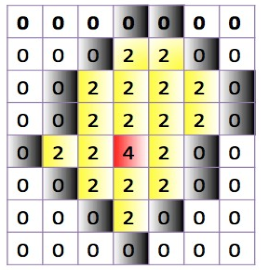
\includegraphics[scale=0.2]{Figures/JES/topoclusterillustration.png}
\end{center}
\end{column}
\hspace{-1cm}
\begin{column}{0.75\textwidth}
\begin{itemize}
\item Calibration clusters\\
$\rightarrow$ non-compensation, out-of-cluster, mat\'eriaux morts
\item JES pour restaurer $R(p_T,\eta)=1$\\
$\rightarrow$ out-of-cone, inefficacit\'es 
\end{itemize}
\end{column}
\end{columns}
\end{block}
}
\end{column}
\pause
\begin{column}{0.35\textwidth}
{
\setbeamercolor{block title}{use=structure,fg=white,bg=purple!75!black}
\setbeamercolor{block body}{use=structure,fg=black,bg=purple!20!white}
\begin{block}{GS {\small (``Global Sequential'')}}
\begin{itemize}
\item EM+JES puis calibration globale
\item cf pages suivantes
\end{itemize}
\end{block}
}
\end{column}
\end{columns}

%\begin{maliste}
%\item 4 calibrations existaient en 2009 :
%\begin{itemize}
%\item EM+JES (prendre du temps pour l'expliquer -> notamment bien dire qu'apre%s reponse = 1, sinon on ne comprendra pas les plots GS)
%\item Global Cell Weighting : GCW
%\item Local Cell Weighting : LCW
%\item Global Sequential Calibration : GS
%\end{itemize}
%\end{maliste}
\end{frame}

\begin{frame}
\frametitle{Calibration Globale S\'equentielle (GS) : principe}
\begin{columns}
\begin{column}{0.75\textwidth}
\begin{small}
\begin{maliste}
\item \'Equipe : Reina Camacho, David Lopez-Mateos, Ariel Schwartzman
\vspace*{0.2cm}
\item \textcolor{magenta}{Eur.Phys.J. C73 (2013) 2304}\\
\textcolor{magenta}{Eur.Phys.J. C73 (2013) 2306}
\vspace*{0.2cm}
\item \EMJES{} supprime dépendance en $\eta$ et $\pt$
\begin{center}
$\rightarrow$ subsiste d'autres dépendances\\
$\rightarrow$ GS les supprime
\end{center}
\item Apr\`es GS : $R(p_T,\eta,x)=1$ ($x$ : variable corr\'el\'ee \`a la r\'eponse)
\vspace*{0.2cm}
\item Int\'er\^et principal : meilleure r\'esolution
\end{maliste}
\end{small}
\end{column}
\begin{column}{0.3\textwidth}
\begin{center}
\hspace*{-0.5cm}
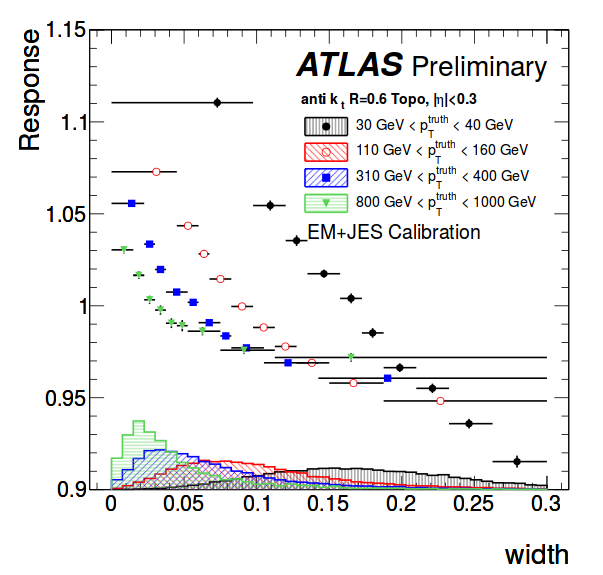
\includegraphics[scale=0.185]{Figures/JES/responseDependenceWidthIllustration.png}
\end{center}
\end{column}
\end{columns}
%\[
%\pt^\GS=\left(\prod\limits_{n=1}^{N}C_n(x_n)\right)\times \pt^\EMJES
%\]
\end{frame}

\begin{frame}
\frametitle{Calibration GS : propri\'et\'es utilis\'ees}
\begin{columns}
\begin{column}{0.6\textwidth}
\begin{center}
\hspace*{-2cm}
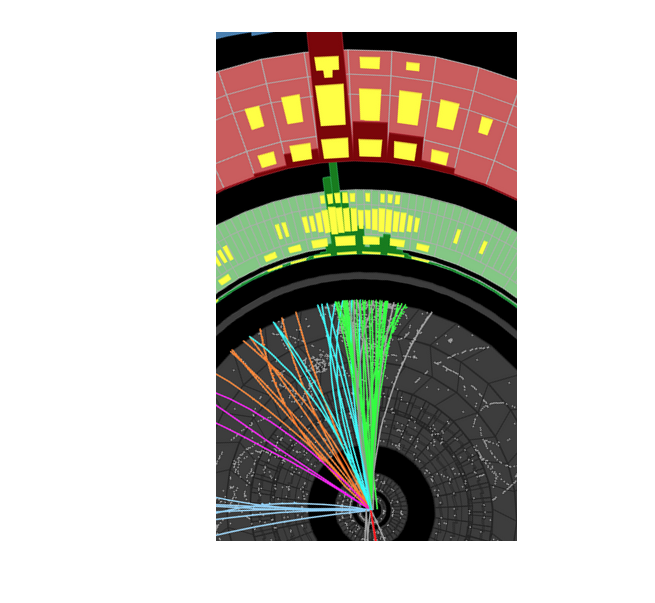
\includegraphics[width=.9\textwidth]{Figures/JES/EventDisplayJet_modified.png}
\hspace*{-1.2cm}
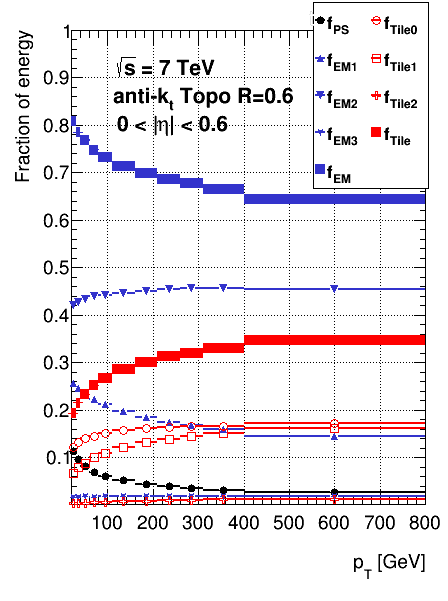
\includegraphics[width=.62\textwidth]{Figures/JES/c_fracs_vs_pt.png}
\end{center}
\end{column}
\begin{column}{0.55\textwidth}
\begin{maliste}
\item Propriétés :
\begin{itemize}
\item longitudinales : $f_{\rm layer}=\frac{E_\EM^{\rm layer}}{E_\EM^{\rm jet}}$
\item transversales : $\width$
\end{itemize}
\vspace*{0.3cm}
\item Plusieurs propri\'et\'es utilis\'ees de mani\`ere s\'equentielle
\[
\pt^\GS=\left(\prod\limits_{n=1}^{N}C_n(x_n)\right)\times \pt^\EMJES
\]
%avant de pouvoir l'appliquer aux autres types d'evts il faut verifier que la calibration est exportable.
\end{maliste}
\end{column}
\end{columns}

%\begin{maliste}
%\item Choix des propri\'et\'es empirique
%\vspace*{0.2cm}
%\item Calibration d\'eriv\'ee pour $0<|\eta|<4,5$ et $p_T<800~$GeV
%$45\times 20 \times 25$ bins en $(\eta,x,p_T)$
%\end{maliste}
\end{frame}

\begin{comment}
\begin{frame}
\frametitle{Calibration GS : effet sur la r\'eponse}
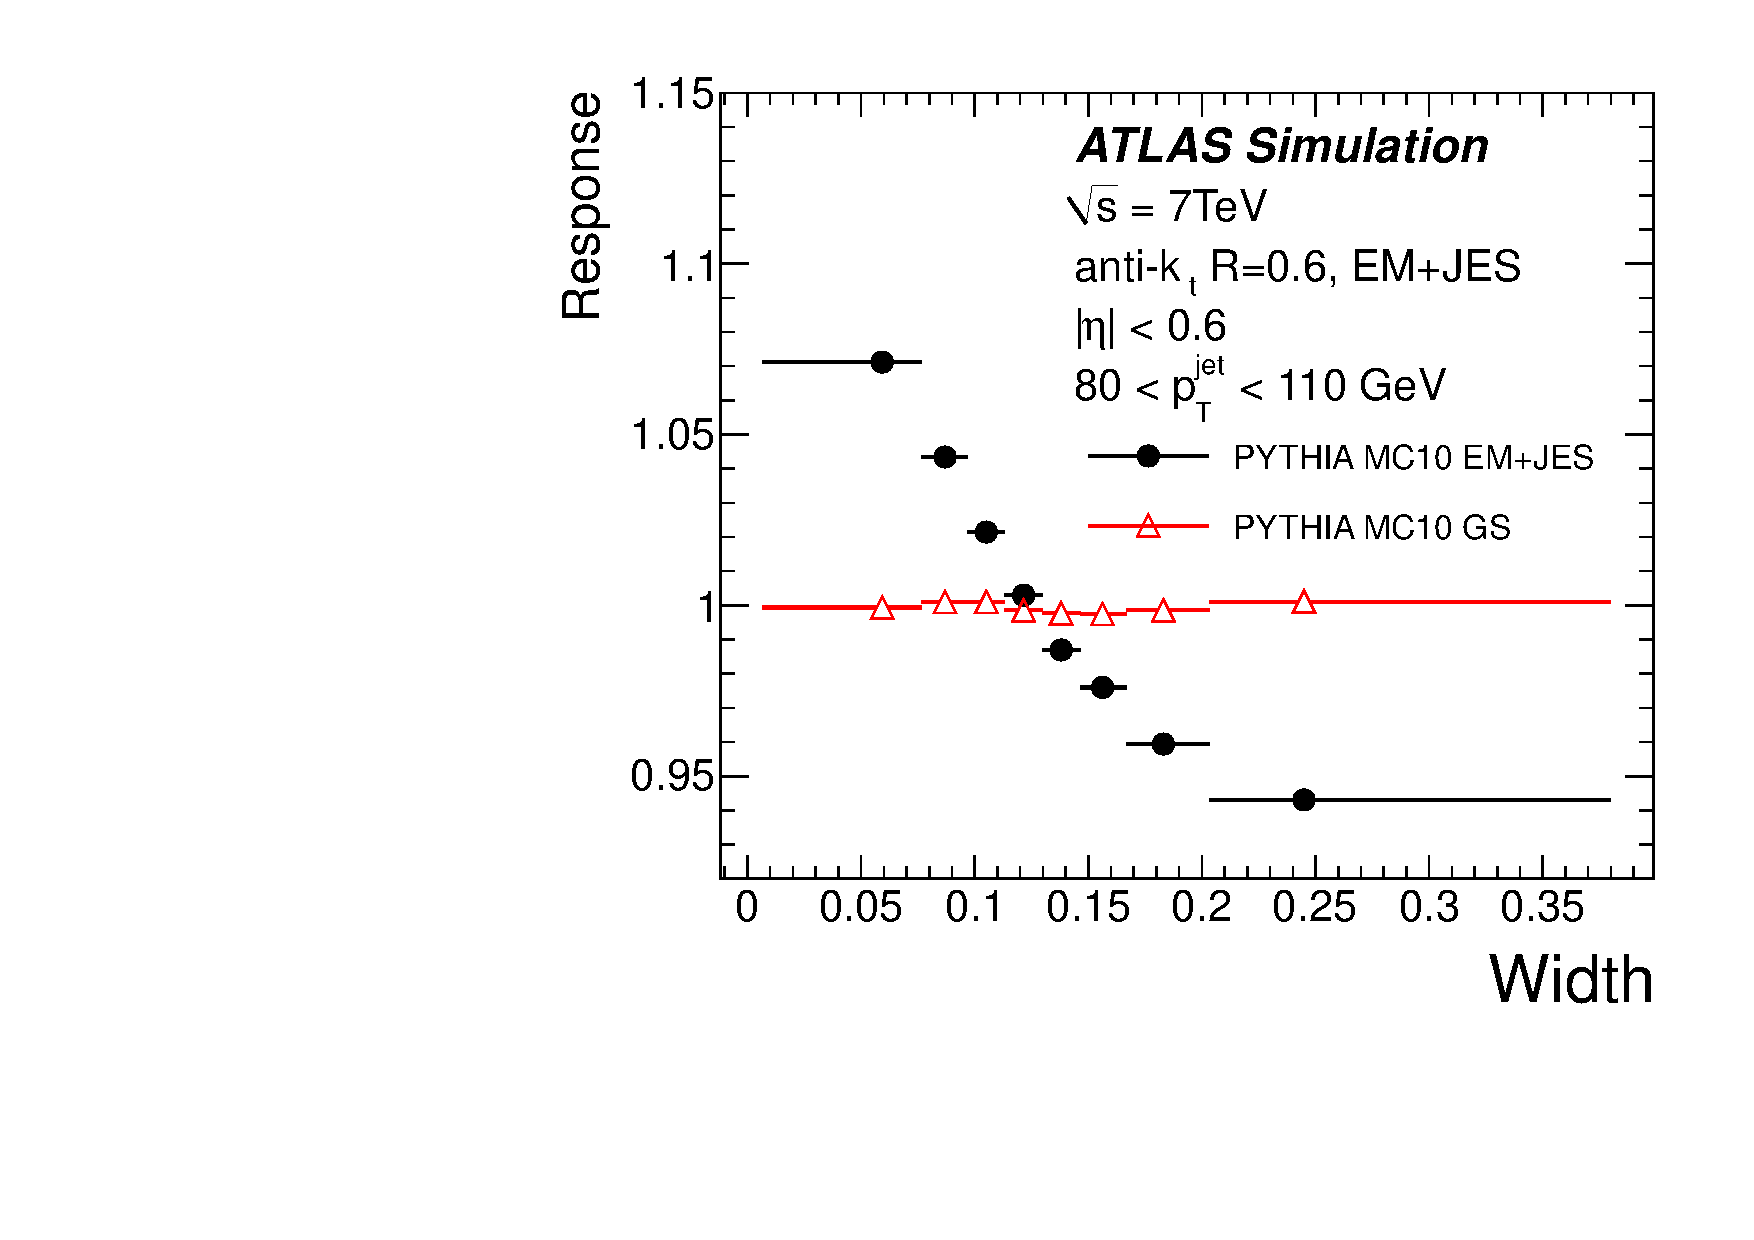
\includegraphics[width=0.5\textwidth]{Figures/JES/fig_46b.pdf}
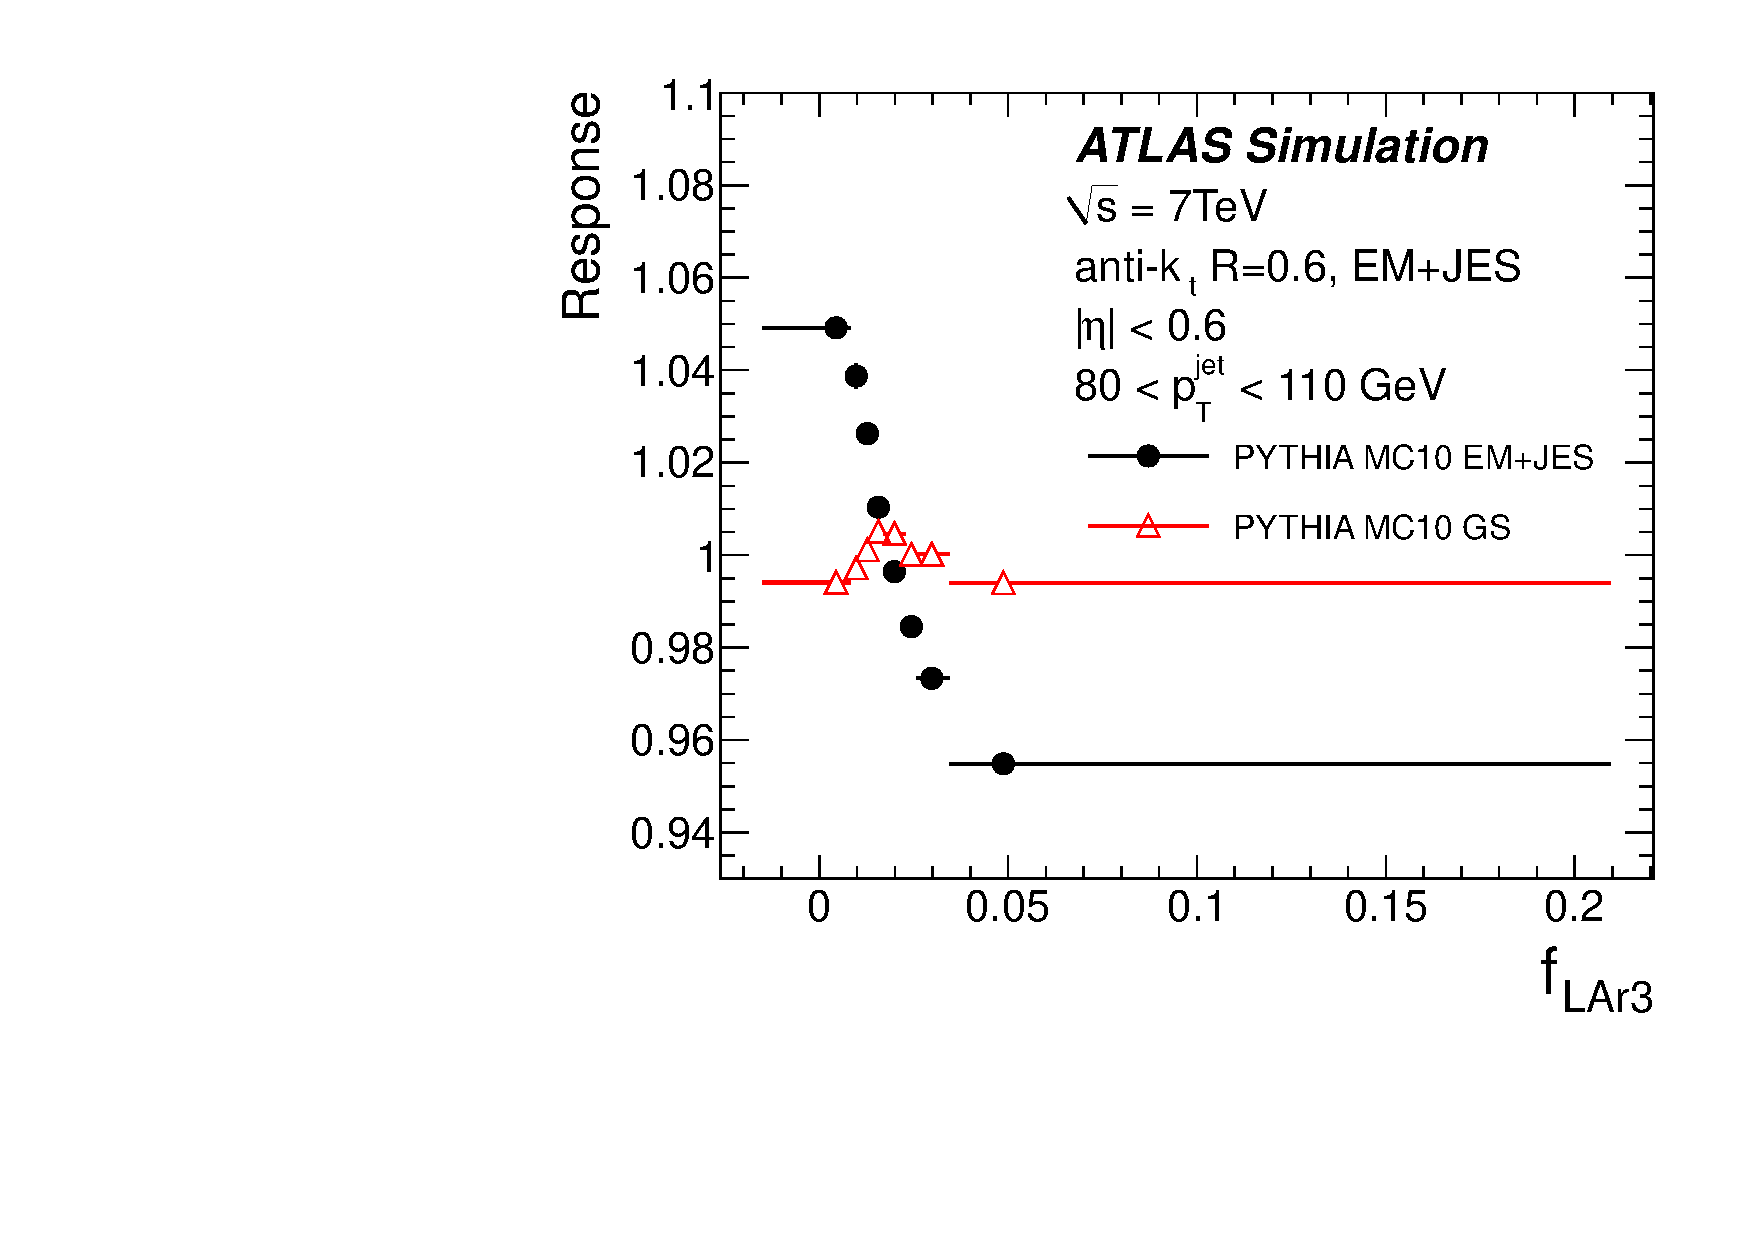
\includegraphics[width=0.5\textwidth]{Figures/JES/fig_46a.pdf}

\vspace*{0.2cm}
\begin{maliste}
\item Quel effet sur la r\'esolution ?\\
\vspace*{0.1cm}
\item Calibration d\'eriv\'ee sur \'echantillon simul\'e multijets\\
\vspace*{0.1cm}
\begin{center}
\textcolor{magenta}{$\rightarrow$ Peut-on l'appliquer \`a d'autres \'echantillons simul\'es et aux donn\'ees ?}
\end{center}
\end{maliste}
\end{frame}
\end{comment}

\begin{frame}
\frametitle{Calibration GS : performances}
\vspace*{-0.8cm}
\begin{maliste}
\item R\'esolution sur simulation et donn\'ees
%\begin{center}
\hspace*{-1cm}
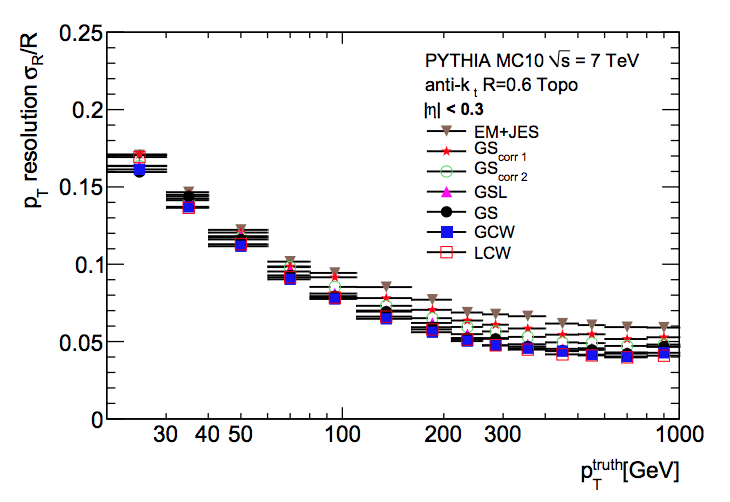
\includegraphics[width=.48\textwidth]{Figures/JES/GSCPerfResolOnMC.png}
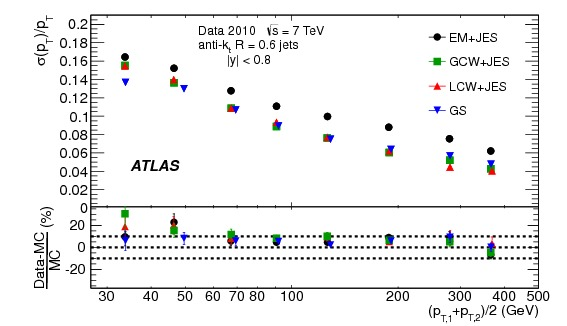
\includegraphics[width=.54\textwidth]{Figures/JES/fig_13a.jpg}
%\end{center}
\begin{center}
$\rightarrow$ Am\'elioration de 20\% \`a 30\% pour $p_T>150$ GeV 
\end{center}

\hspace*{7cm}
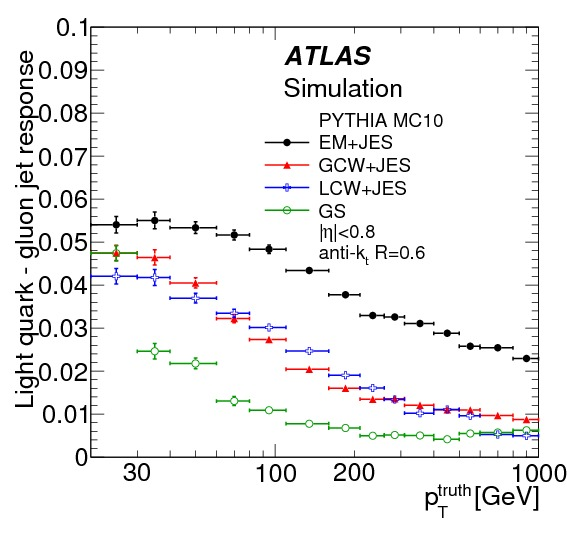
\includegraphics[width=.35\textwidth]{Figures/JES/fig_78a.jpg}
\vspace*{-3.5cm}
\item D\'ependance avec la saveur du jet\\
\vspace*{0.1cm}
$\rightarrow$ r\'eponse diff\'erente pour quarks et gluons\\
\vspace*{0.1cm}
$\rightarrow$ r\'eponse moyenne d\'epend de la composition\\
en saveur
\end{maliste}
\end{frame}

\begin{frame}
\frametitle{Calibration GS : validation sur les données}
\vspace*{-0.2cm}
\begin{maliste}
\item Calibration GS peut-\^etre d\'eriv\'ee sur les donn\'ees r\'eelles

\vspace*{0.3cm}
\begin{columns}
\begin{column}{0.5\textwidth}
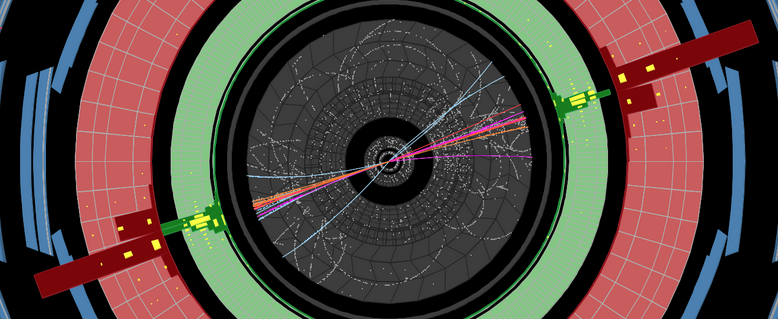
\includegraphics[width=1\textwidth]{Figures/JES/DijetsEventDisplay.png}
\end{column}
\begin{column}{0.5\textwidth}
\[A(x)=2\frac{p_T^\text{probe}(x)-p_T^\text{ref}}{p_T^\text{probe}(x)+p_T^\text{ref}}\]
\vspace*{-0.1cm}
\[
\hspace*{1cm}
\Rightarrow
\left<R(x)\right>\simeq\frac{2+\left<A(x)\right>}{2-\left<A(x)\right)}
\]
\end{column}
\end{columns}
\vspace*{0.2cm}
\item M\'ethode valid\'ee sur simulation puis appliqu\'ee aux donn\'ees
\vspace*{-0.1cm}
\end{maliste}
\begin{center}
%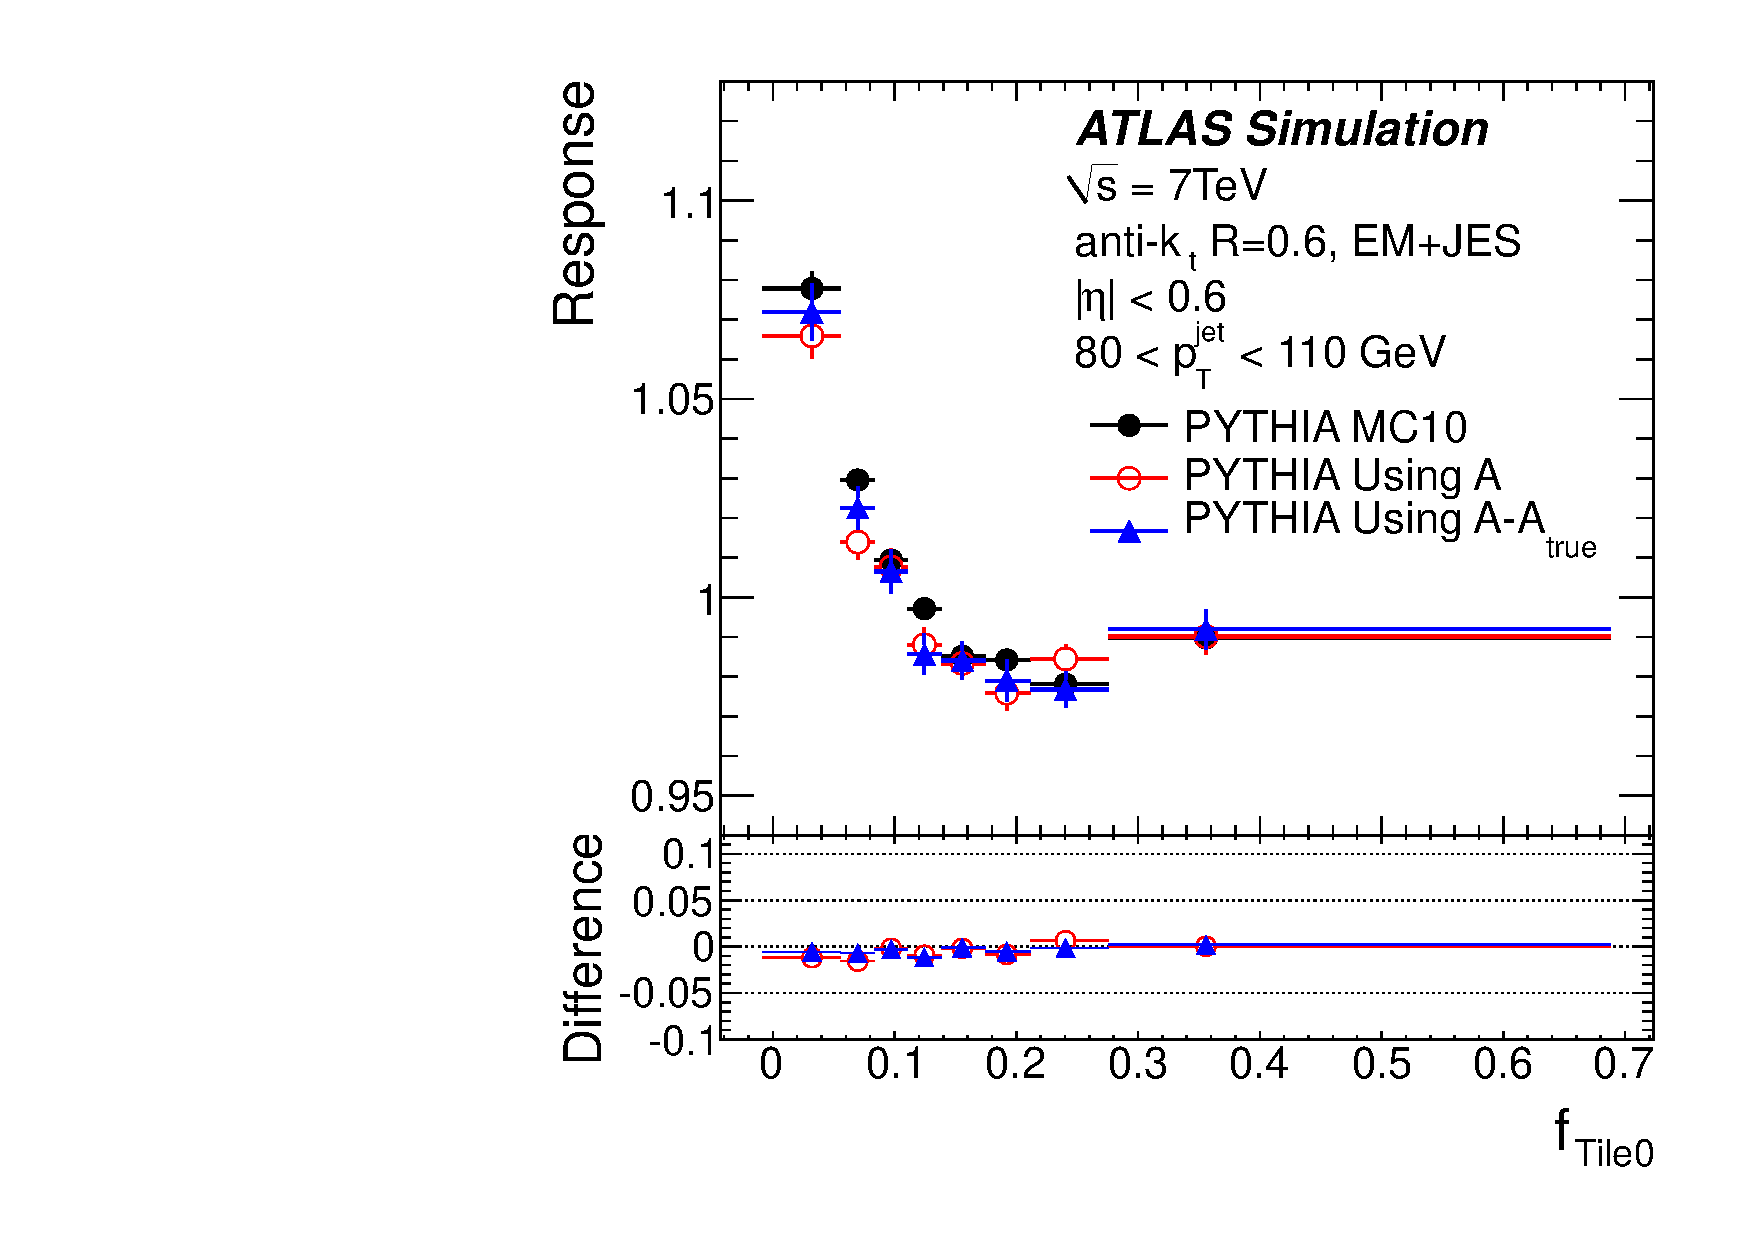
\includegraphics[width=.4\textwidth]{Figures/JES/fig_47c.pdf}
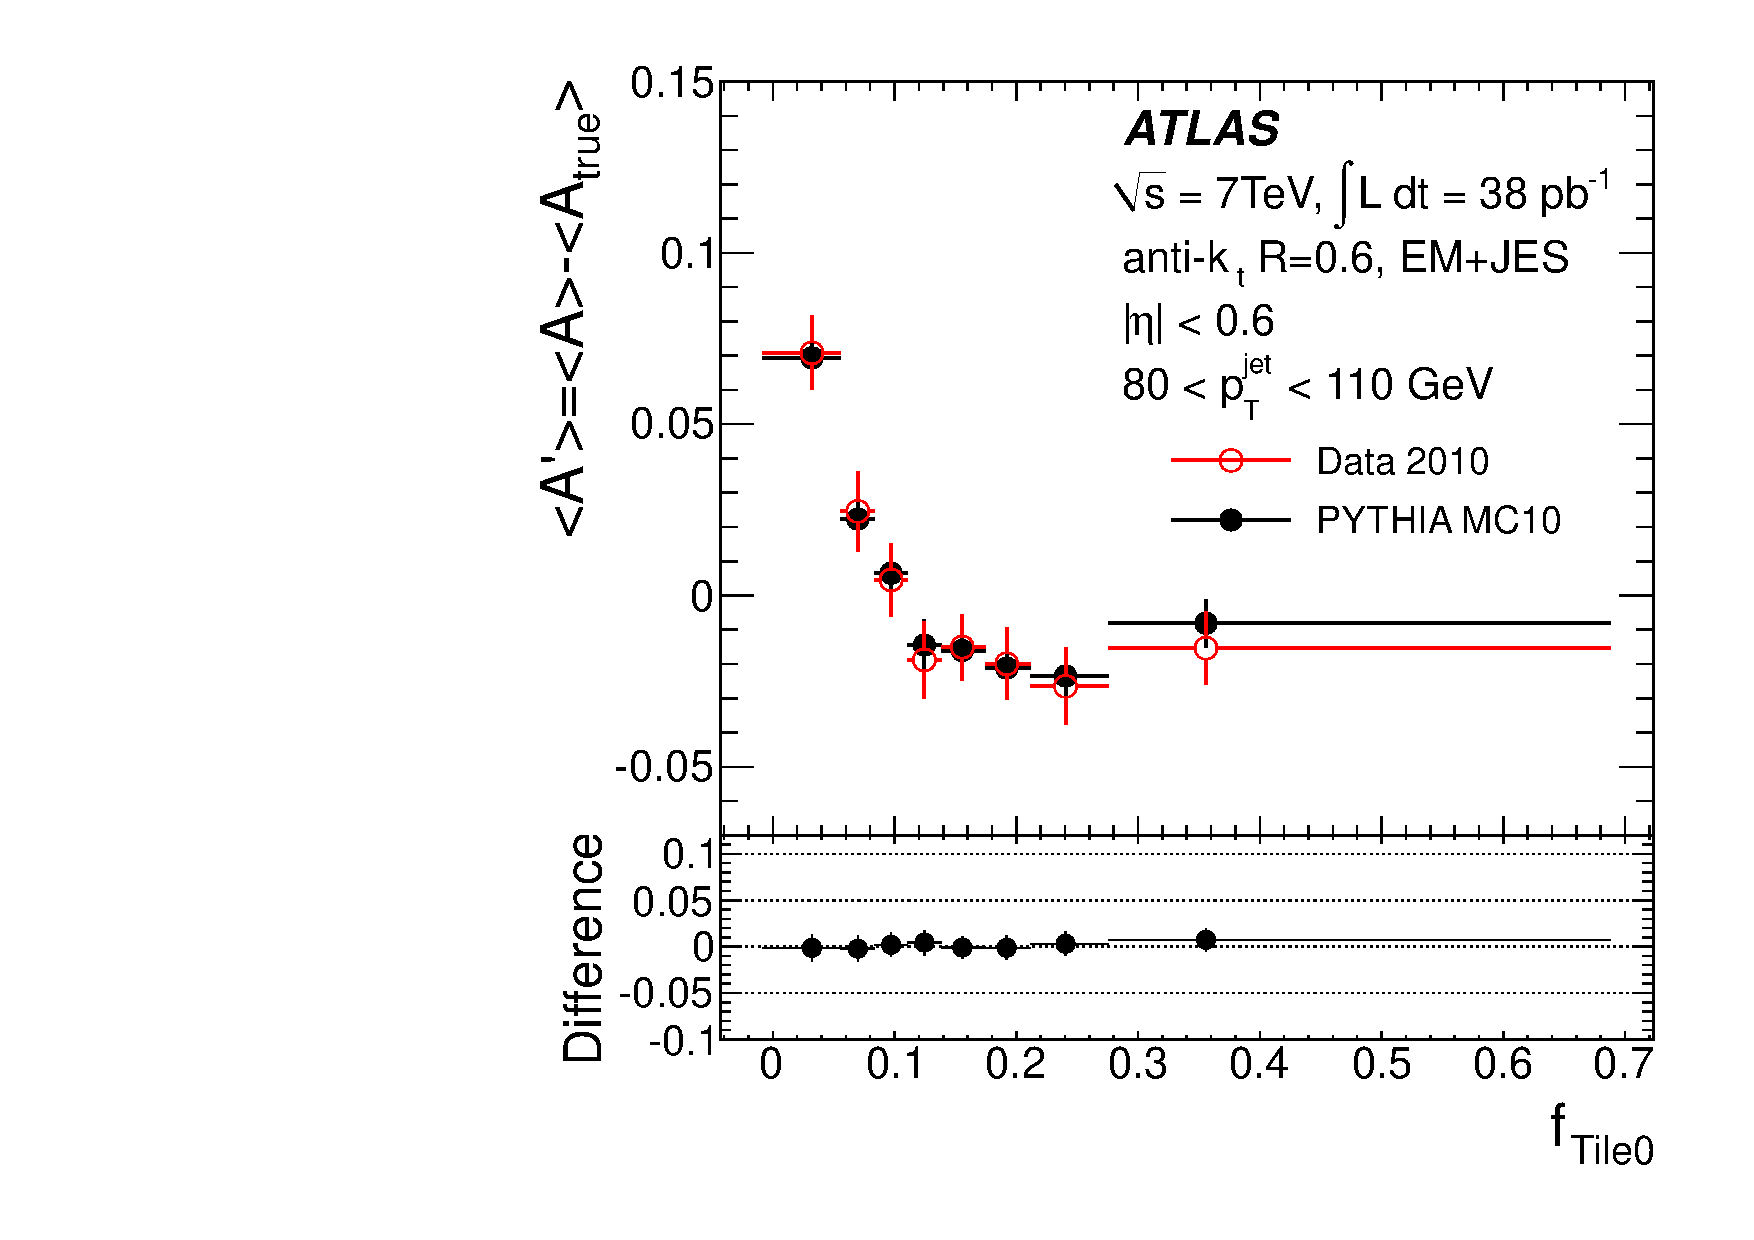
\includegraphics[width=.4\textwidth]{Figures/JES/fig_49c.pdf}
\end{center}
\vspace*{-0.35cm}
\begin{center}
\textcolor{magenta}{$\rightarrow$ calibration GS valid\'ee avec 38~pb$^{-1}$ !}
\end{center}
\end{frame}

\begin{frame}
\frametitle{Calibration GS : diff\'erences donn\'ees/simulation}

\begin{maliste}
\item Erreurs sur propri\'et\'es $\Rightarrow$ Incertitude sur r\'eponse moyenne
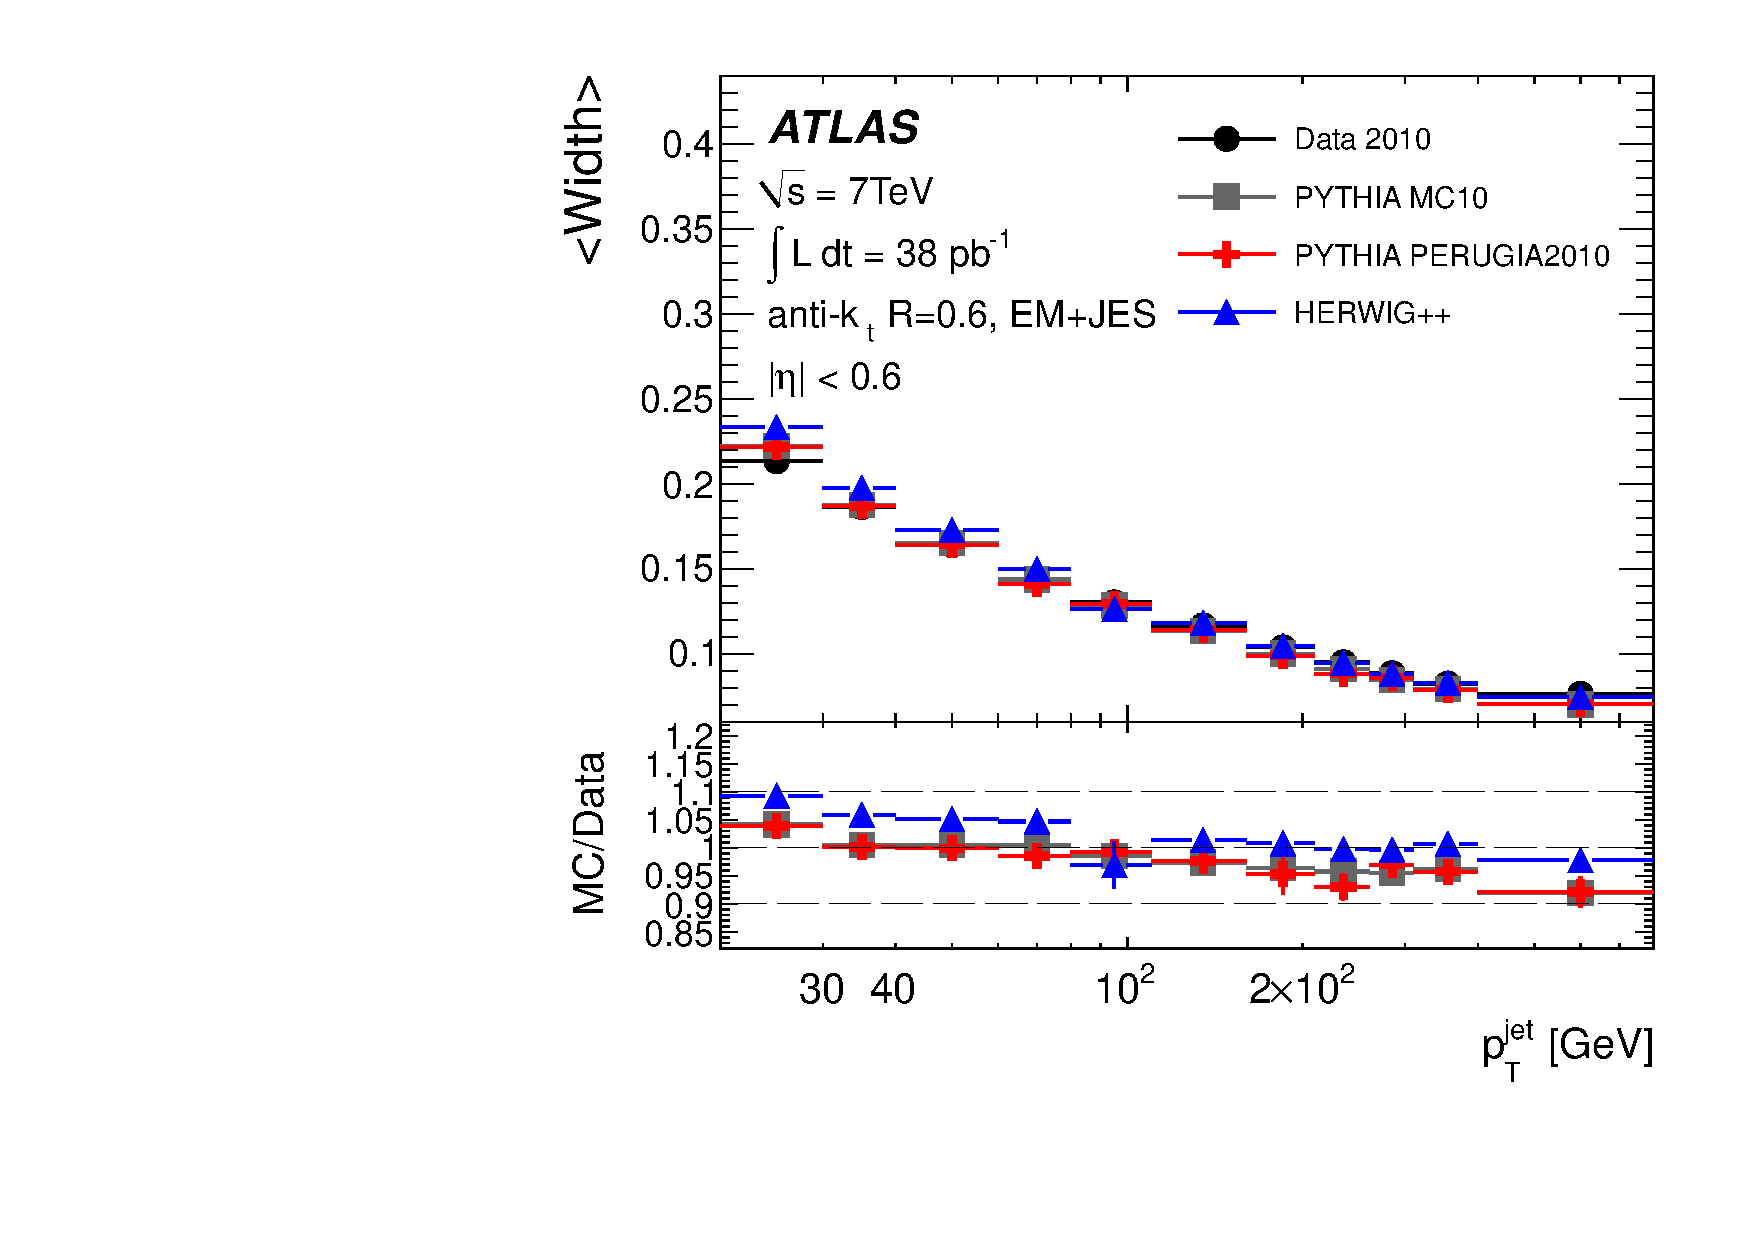
\includegraphics[width=.37\textwidth]{Figures/JES/fig_50c.pdf}
\quad
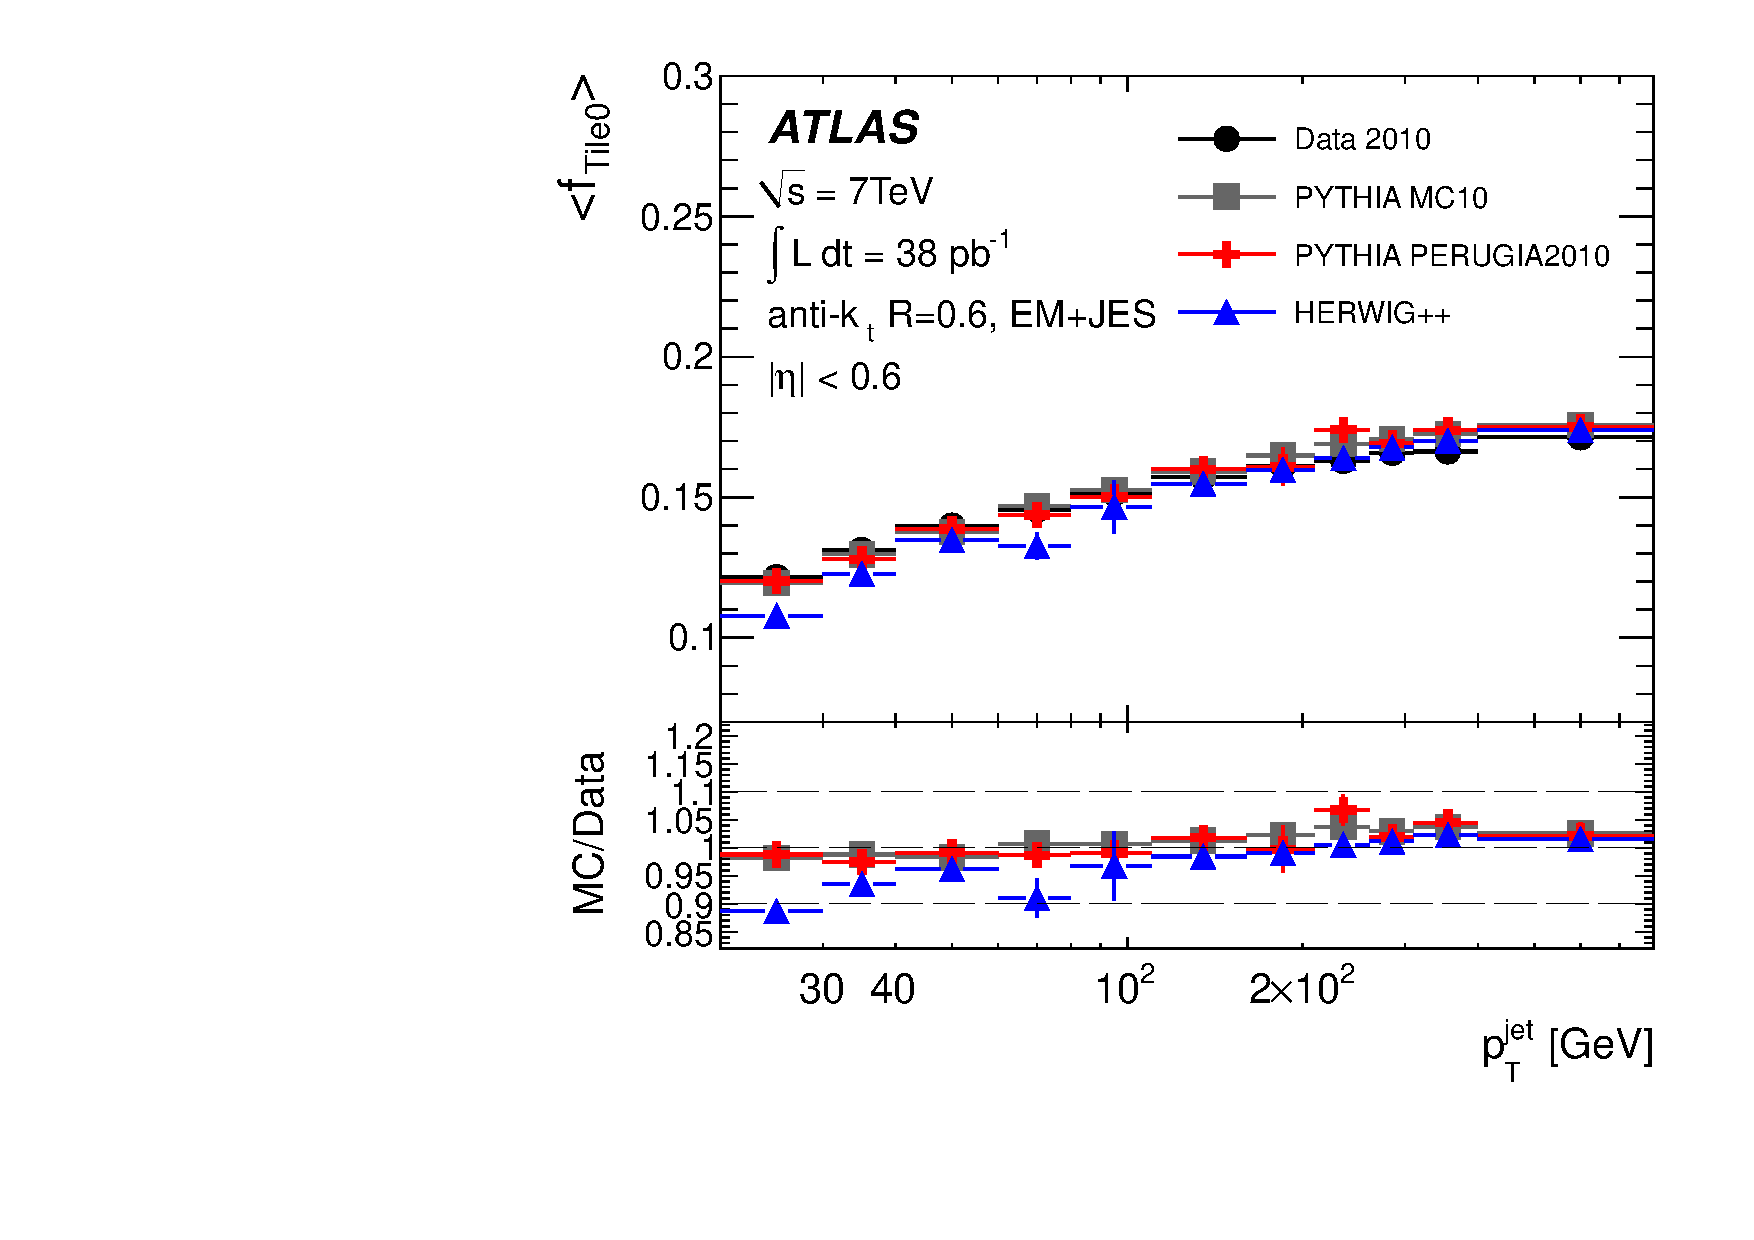
\includegraphics[width=.37\textwidth]{Figures/JES/fig_50d.pdf}
\end{maliste}

\vspace*{-0.5cm}
\begin{columns}
\begin{column}{0.3\textwidth}
\vspace{-0.5cm}
\begin{center}
%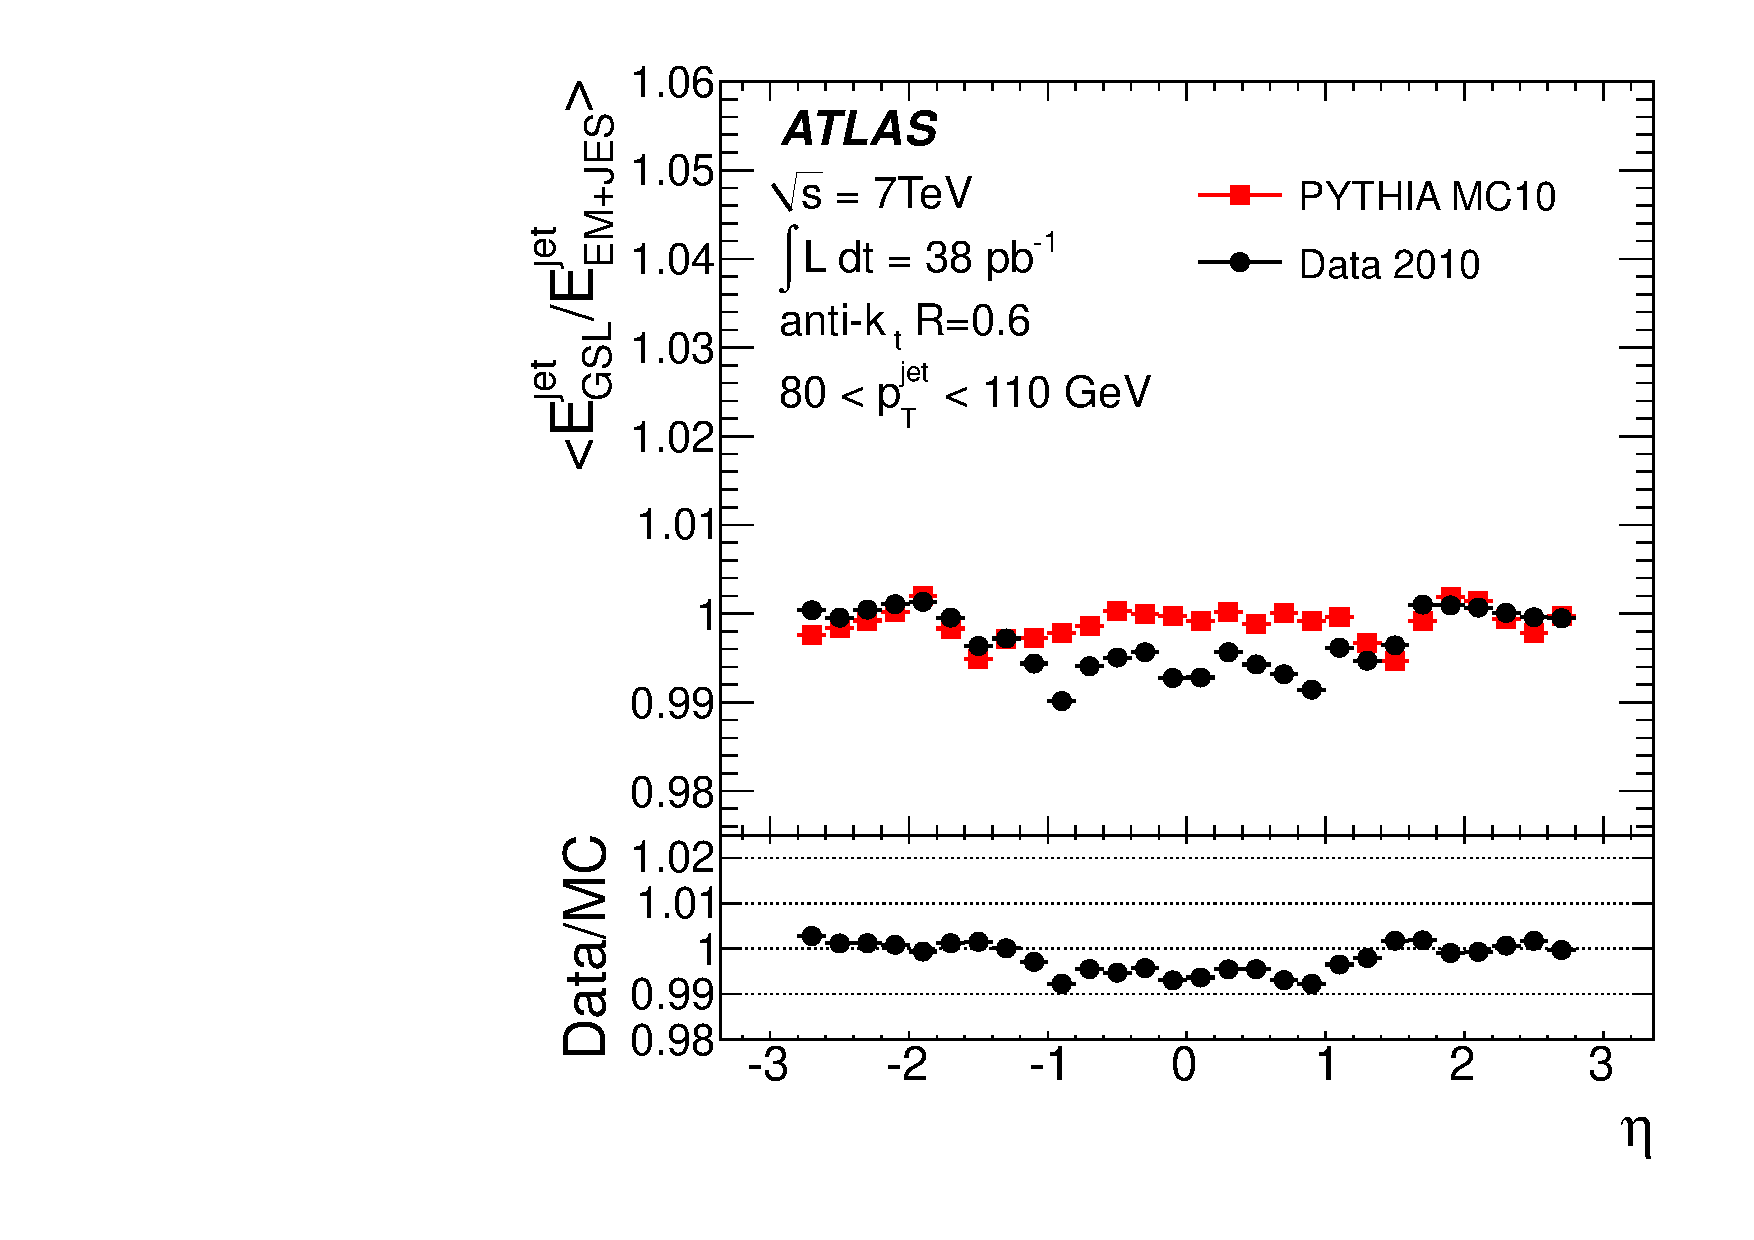
\includegraphics[width=0.7\textwidth]{Figures/JES/fig_51c.pdf}
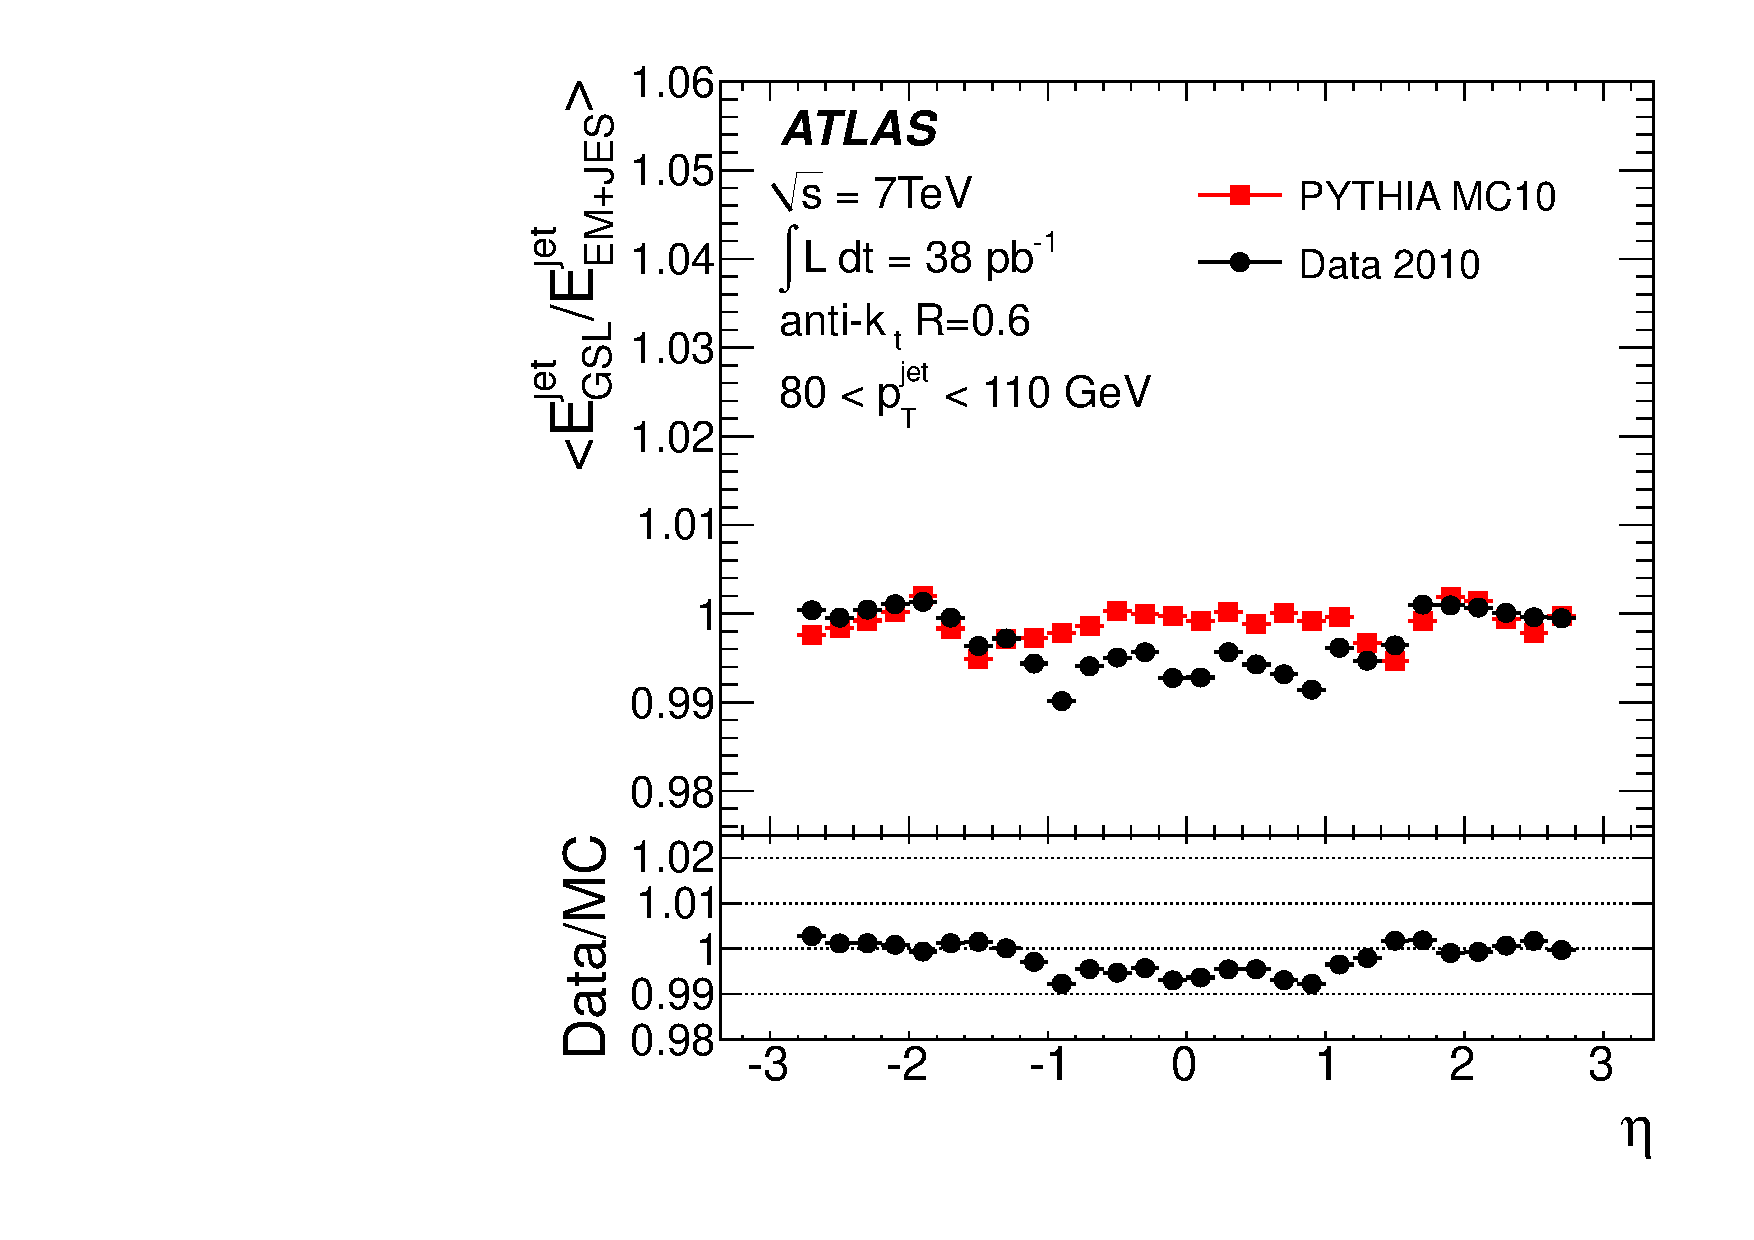
\includegraphics[width=1.2\textwidth]{Figures/JES/fig_51c.pdf}
\end{center}
\end{column}
\begin{column}{0.6\textwidth}
\begin{maliste}
\item[$\rightarrow$] Incertitude estim\'ee sur evts multi-jets, $\gamma$+jets, sans et avec pile-up
\vspace*{0.3cm}
\item[$\rightarrow$] R\'esultat : incertitude syst. $\simeq 1$\%
\vspace*{0.3cm}
\item[$\Rightarrow$] GS induit une d\'egradation minime de l'\'echelle en \'energie
\end{maliste}
\end{column}
\end{columns}
\end{frame}

\begin{frame}
\frametitle{Ce qu'il reste}
\begin{maliste}
%\item Calibration des jets sur les premi\`eres donn\'ees : EM+JES et GS
%\vspace*{0.5cm}
\item Nous avons montr\'e que GS est une calibration : 
\begin{itemize}
\item relativement simple \`a mettre en \oe uvre
\item performante 
\item facile à valider sur les donn\'ees
\end{itemize}
%\vspace*{0.2cm}
\hspace*{7cm}
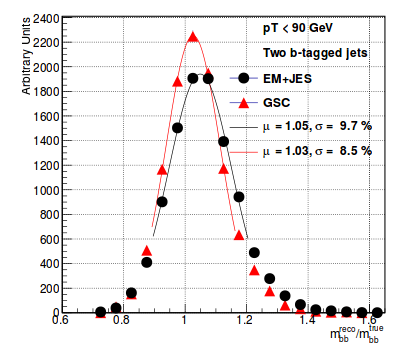
\includegraphics[width=0.33\textwidth]{Figures/JES/HbbPlotMbbVsMbbtrue.png}
%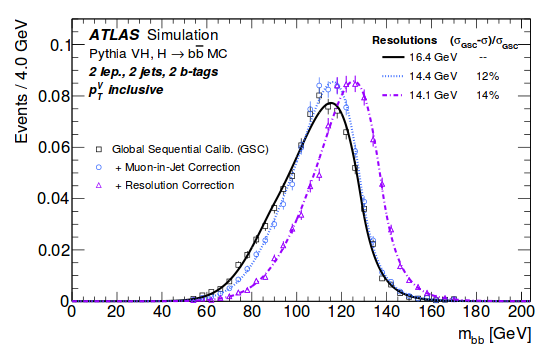
\includegraphics[width=0.4\textwidth]{Figures/JES/MbbPlotPublic.png}
\vspace*{-3.cm}
%\item Notre travail = preuve de concept
\vspace*{0.5cm}
\item GS utilis\'ee pour la premi\`ere fois pour \\la recherche $H\rightarrow b\bar{b}$
\vspace*{0.5cm}
\item \'Etat actuel dans ATLAS :
\vspace*{0.3cm}
\begin{itemize}
\item GS utilis\'ee en combinaison avec LCW
\hspace*{-0.8cm}
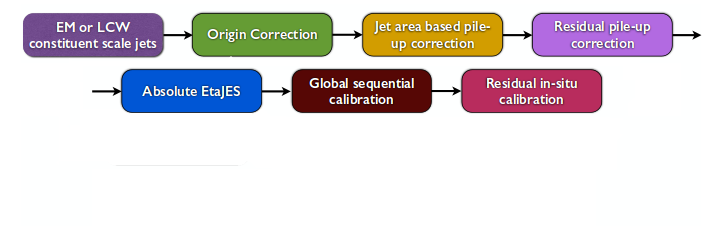
\includegraphics[width=1\textwidth]{Figures/JES/CurrentATLASJetCalib_modified.png}
\end{itemize}
\end{maliste}
\end{frame}

